\documentclass{elegantbook}
\usepackage[square,numbers,sort&compress]{natbib}
\newcommand{\upcite}[1]{\textsuperscript{\textsuperscript{\cite{#1}}}}
\usepackage{multirow}
\usepackage{color}
\usepackage{tikz}
\usepackage{algorithm}
\usepackage{algorithmic}
\renewcommand{\algorithmicrequire}{ \textbf{Input:}} 
\renewcommand{\algorithmicensure}{ \textbf{Output:}} 
\usetikzlibrary{shapes.geometric, arrows}
\tikzstyle{startstop} = [rectangle, rounded corners, minimum width = 2cm, minimum height=1cm,text centered, draw = black, fill = red!40]
\tikzstyle{acti} = [rectangle, trapezium left angle=70, trapezium right angle=110, minimum width=5cm, minimum height=0.5cm, text centered, draw=black, fill = blue!40]
\tikzstyle{pool} = [rectangle, trapezium left angle=70, trapezium right angle=110, minimum width=2cm, minimum height=0.5cm, text centered, draw=black, fill = purple!40]
\tikzstyle{process} = [rectangle, minimum width=3cm, minimum height=1cm, text centered, draw=black, fill = green!50]
\tikzstyle{conv} = [rectangle, minimum width=3cm, minimum height=1cm, text centered, draw=black, fill = magenta!50]
\tikzstyle{loss} = [rectangle, rounded corners, minimum width = 2cm, minimum height=1cm,text centered, draw = black, fill = yellow!40]
\tikzstyle{arrow} = [->,>=stealth]

% title info
\title{Deep Learning}
\subtitle{MNIST Digits Classification using PyTorch}
% bio info
\author{Yantian Luo}
\institute{Electronic Engineering}
\version{2018310742}
\date{\today}
\logo{logo.png}
\cover{cover.jpg}

\begin{document}

\maketitle
\tableofcontents
\mainmatter
\hypersetup{pageanchor=true}
% add preface chapter here if needed
\chapter{Introduction}
MNIST digits dataset is a widely used database for image classification in machine learning field. It contains 60,000 training samples and 10,000 testing samples. Each sample is a $784\times1$ column vector, which is transformed from an original $28\times28$ pixels grayscale image.

In this homework, we will continue working on MNIST digits classification problem by utilizing Pytorch framework to implement neural networks. Pytorch provides good abstraction for different modules, and its auto-differentiation feature can save us from the backward details.

\chapter{Algorithm Design}
In the last two homework, we have implement Linear layer, activation layer, convolution layer and loss layer, in this homework, we only implement an important technique discovered recently and utilize Pytorch framework to implement others.

%\section{Training phase}
For every input $x_i$ across a mini-batch, the output can be computed as :
\begin{equation}
BN(x_i)=\gamma \cdot \frac{x_i-\mu_B}{\sqrt{\sigma^2+\epsilon}}+\beta
\end{equation}
where $\gamma$ and $\beta$ are learnable parameters, $\mu_B$ is the mean of the mini-batch and $\sigma^2$ is the variance of the mini-batch.

%\section{Evaluation phase}
When we test our samples one by one, the normalization may not work because we don’t have mini- batch concept this time. Therefore, during training we should keep running estimates of its computed mean and variance, which are then used for normalization during evaluation. The running estimates are kept with a default momentum of 0.9, which can be mathematically expressed as
\begin{equation}
\begin{aligned}
\hat{\mu}_{new} &= momentum \times \hat{\mu} + (1-momentum)\times \mu_t \\
\hat{\sigma}_{new}^2 &= momentum \times \hat{\sigma}^2 + (1-momentum)\times \sigma_t^2
\end{aligned}
\end{equation}
where where $\hat{\mu},\hat{\sigma}^2$ are the estimated statistic and $\mu_t,\sigma_t^2$ is the new observed value. 

\chapter{Results}

\section{MLP}
In this section, we use MLP to work on MNIST digits classification. The network structure is shown in Figure \ref{fig1}. And we also compare the results of MLP with BatchNorm and the results without the BatchNorm.
\begin{figure}[htbp]
	\centering
	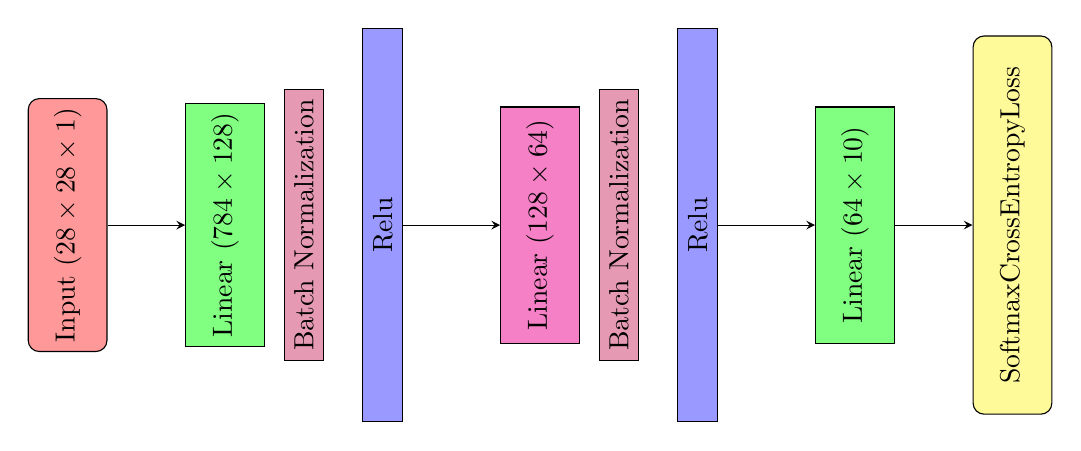
\begin{tikzpicture}
	\node (start) [startstop, rotate=90] {Input ($28\times28\times 1$)};
	\node (linear1) [process, rotate=90, below of=start, yshift=-1cm] {Linear ($784\times 128$)};
	\node (bn1) [pool, rotate=90, below of=linear1] {Batch Normalization};
	\node (acti1) [acti, rotate=90, below of=bn1] {Relu};
	\node (linear2) [conv, rotate=90, below of=acti1, yshift=-1cm] {Linear ($128\times 64$)};
	\node (bn2) [pool, rotate=90, below of=linear2] {Batch Normalization};
	\node (acti2) [acti, rotate=90, below of=bn2] {Relu};
	\node (linear3) [process, rotate=90, below of=acti2, yshift=-1cm] {Linear ($64\times 10$)};
	\node (loss) [loss, rotate=90, below of=linear3, yshift=-1cm, text width=13em] {SoftmaxCrossEntropyLoss};
	
	\draw [arrow](start) -- (linear1);
	%		\draw [arrow](conv1) -- (acti1);
	%		\draw [arrow](acti1) -- (pool1);
	\draw [arrow](acti1) -- (linear2);
	%		\draw [arrow](conv2) -- (acti2);
	%		\draw [arrow](acti2) -- (pool2);
	\draw [arrow](acti2) -- (linear3);
	\draw [arrow](linear3) -- (loss);
	\end{tikzpicture}
	\caption{\label{fig1}MLP Network Structure}
\end{figure}

The training arguments is as follow:

\begin{lstlisting}[frame=single,language=python]  
config = {
'learning_rate': 0.1,
'weight_decay': 0.0001,
'momentum': 0.9,
'batch_size': 100,
'max_epoch': 100,
'disp_freq': 50,
}
\end{lstlisting}

\subsection{Results with BatchNorm}
From the results we can find that only after 5000 iterations, the training accuracy is up to $90\%$, which is very fast converging, and after one epoch, the test accuracy can up to $96.56\%$. Then we draw the train accuracy curve and train loss curve as shown in Figure \ref{trainres11} and we draw the test accuracy curve and test loss curve with respect to epoch as shown in Figure \ref{testres11}.

\begin{figure}[!h]
	\centering
	\begin{minipage}[t]{0.48\textwidth}
		\centering
		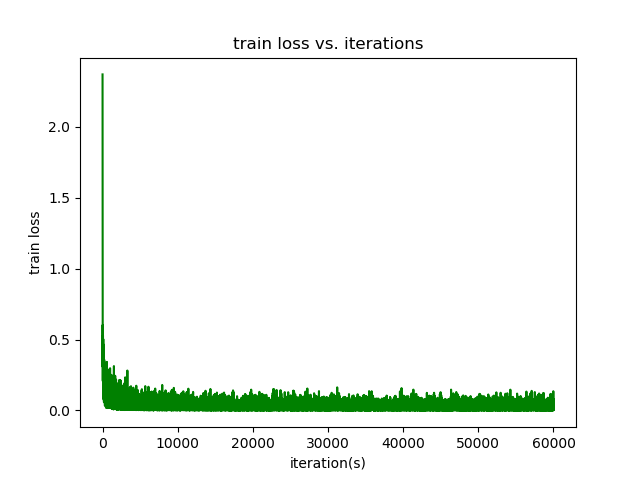
\includegraphics[width=\textwidth]{../results/trainloss11}
	\end{minipage}
	\begin{minipage}[t]{0.48\textwidth}
		\centering
		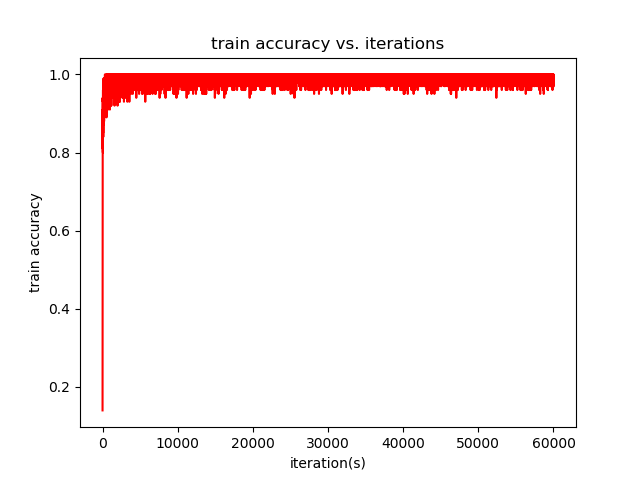
\includegraphics[width=\textwidth]{../results/trainacc11}
	\end{minipage}
	\caption{\label{trainres11}train loss curve and train accuracy curve using MLP with BatchNorm}
\end{figure}

\begin{figure}[!h]
	\centering
	\begin{minipage}[t]{0.48\textwidth}
		\centering
		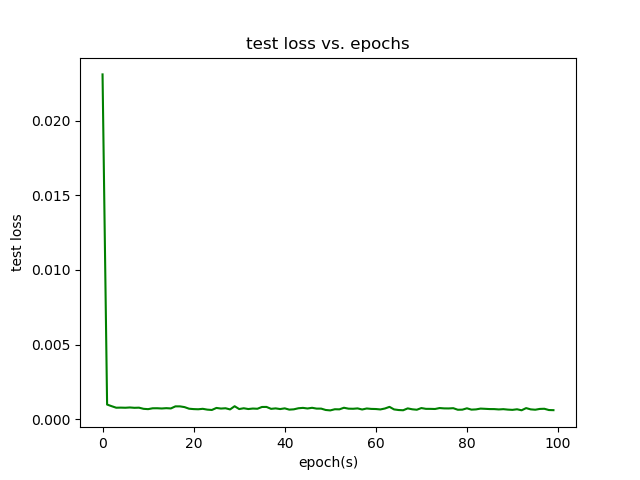
\includegraphics[width=\textwidth]{../results/testloss11}
	\end{minipage}
	\begin{minipage}[t]{0.48\textwidth}
		\centering
		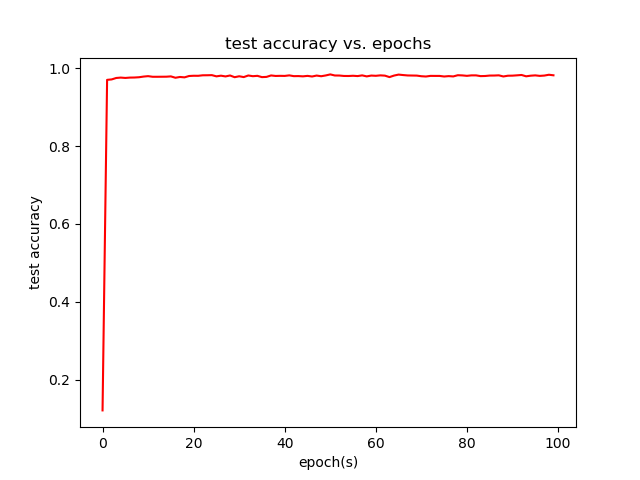
\includegraphics[width=\textwidth]{../results/testacc11}
	\end{minipage}
	\caption{\label{testres11}test loss curve and test accuracy curve using MLP with BatchNorm}
\end{figure}

\subsection{Results without BatchNorm}
From the results we can find that after 15000 iterations, the training accuracy can up to $90\%$, which is slower than the results with BatchNorm, and after one epoch, the test accuracy can up to $95.46\%$, which is also smaller than the results with BatchNorm. Then we draw the train accuracy curve and train loss curve as shown in Figure \ref{trainres12} and we draw the test accuracy curve and test loss curve with respect to epoch as shown in Figure \ref{testres12}.

\begin{figure}[!h]
	\centering
	\begin{minipage}[t]{0.48\textwidth}
		\centering
		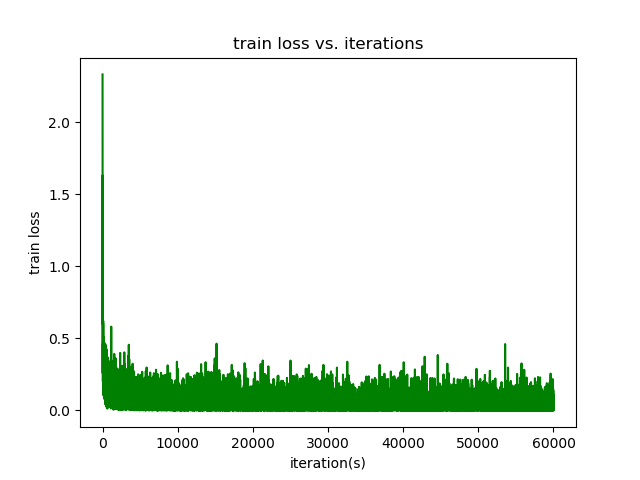
\includegraphics[width=\textwidth]{../results/trainloss12}
	\end{minipage}
	\begin{minipage}[t]{0.48\textwidth}
		\centering
		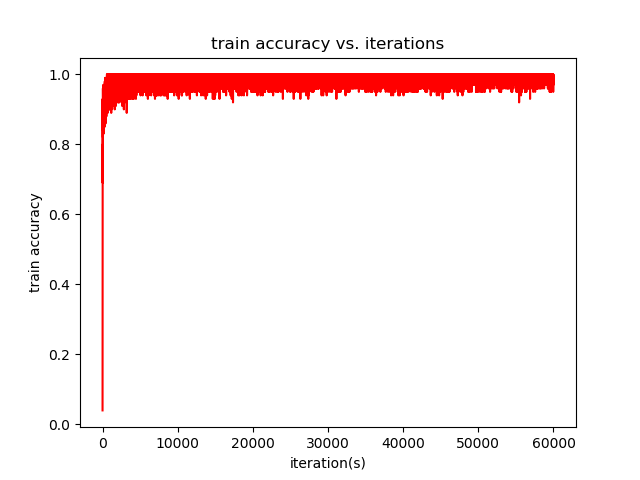
\includegraphics[width=\textwidth]{../results/trainacc12}
	\end{minipage}
	\caption{\label{trainres12}train loss curve and train accuracy curve using MLP without BatchNorm}
\end{figure}

\begin{figure}[!h]
	\centering
	\begin{minipage}[t]{0.48\textwidth}
		\centering
		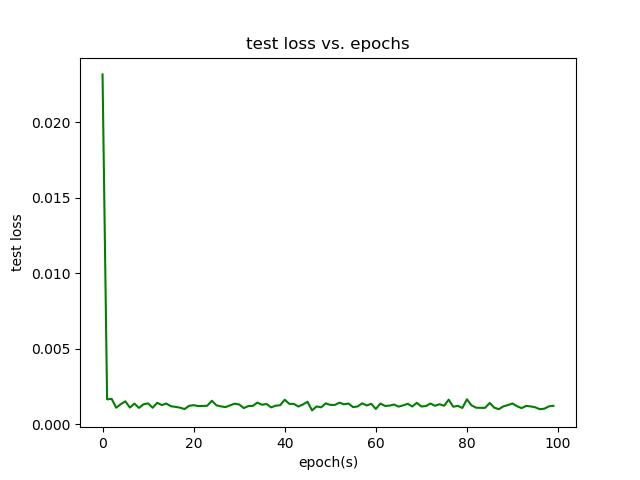
\includegraphics[width=\textwidth]{../results/testloss12}
	\end{minipage}
	\begin{minipage}[t]{0.48\textwidth}
		\centering
		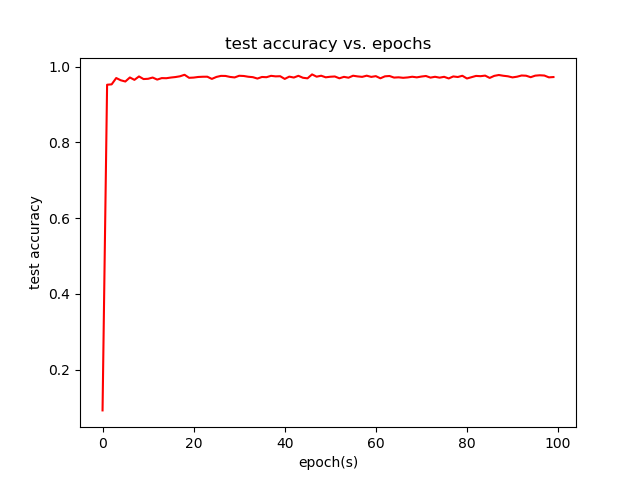
\includegraphics[width=\textwidth]{../results/testacc12}
	\end{minipage}
	\caption{\label{testres12}test loss curve and test accuracy curve using MLP without BatchNorm}
\end{figure}

\subsection{Comparisons}
Here we list the comparisons of the last two results as shown in Table \ref{tab1}. From the table, we can find that:
\begin{itemize}
	\item The result of MLP with BN has faster converging speed than MLP without BN;
	\item The test accuracy of MLP with BN is also bigger than MLP without BN, and the test loss of MLP with BN is less than MLP without BN;
	\item The parameters number of MLP with BN is a little more than MLP without BN, because the BN layer has trainable parameters, but it's a very little number;
	\item The training time of two cases is close and MLP without BN has a little shorter training time than MLP with BN because MLP with BN has a little more parameters than MLP without BN;
\end{itemize}
Therefore, we can find, using BatchNorm in MLP is better than normal MLP.
\begin{table}[!h]
	\centering
	\caption{\label{tab1}The comparisons of the results with BatchNorm and without BatchNorm}
	\begin{tabular}{|c|c|c|c|c|c|}
		\hline
		Cases & Converge speed & test Acc & test loss & training time & \#(parameters) \\
		\hline
		With BN & faster & 0.983 & 0.0006 & 17min & 109,568 \\
		\hline
		Without BN & slower & 0.976 & 0.0010 & 14min & 109,184 \\
		\hline
	\end{tabular}
\end{table}

\section{CNN}
In this section, we use CNN to work on MNIST digits classification. The network structure is shown in Figure \ref{fig2}. And we also compare the results of CNN with BatchNorm and the results without the BatchNorm.
\begin{figure}[htbp]
	\centering
	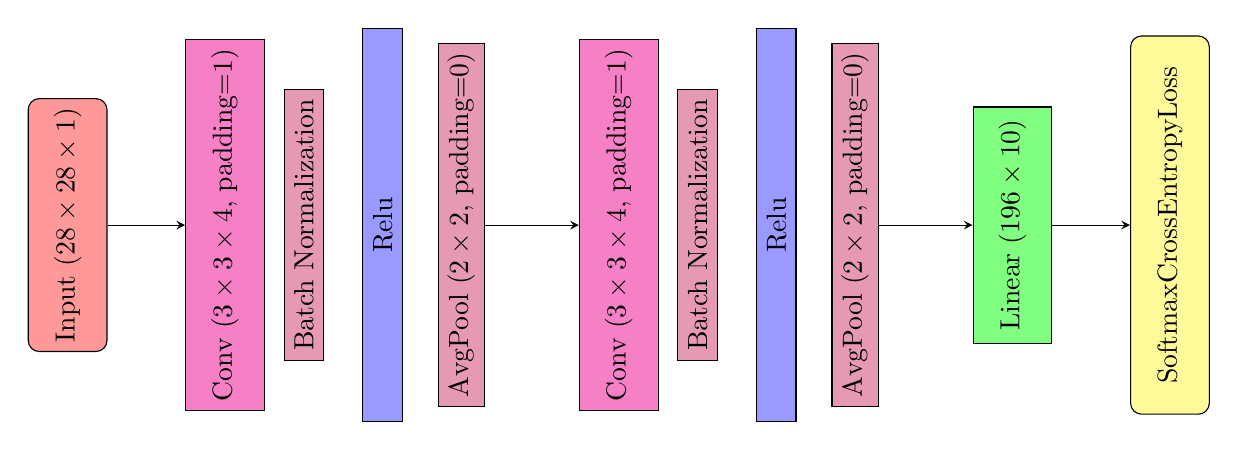
\begin{tikzpicture}
	\node (start) [startstop, rotate=90] {Input ($28\times28\times 1$)};
	\node (conv1) [conv, rotate=90, below of=start, yshift=-1cm] {Conv ($3\times3\times 4$, padding=1)};
	\node (bn1) [pool, rotate=90, below of=conv1] {Batch Normalization};
	\node (acti1) [acti, rotate=90, below of=bn1] {Relu};
	\node (pool1) [pool, rotate=90, below of=acti1] {AvgPool ($2\times2$, padding=0)};
	\node (conv2) [conv, rotate=90, below of=pool1, yshift=-1cm] {Conv ($3\times3\times 4$, padding=1)};
	\node (bn2) [pool, rotate=90, below of=conv2] {Batch Normalization};
	\node (acti2) [acti, rotate=90, below of=bn2] {Relu};
	\node (pool2) [pool, rotate=90, below of=acti2] {AvgPool ($2\times2$, padding=0)};
	\node (linear) [process, rotate=90, below of=pool2, yshift=-1cm] {Linear ($196\times10$)};
	\node (loss) [loss, rotate=90, below of=linear, yshift=-1cm, text width=13em] {SoftmaxCrossEntropyLoss};
	
	\draw [arrow](start) -- (conv1);
	%		\draw [arrow](conv1) -- (acti1);
	%		\draw [arrow](acti1) -- (pool1);
	\draw [arrow](pool1) -- (conv2);
	%		\draw [arrow](conv2) -- (acti2);
	%		\draw [arrow](acti2) -- (pool2);
	\draw [arrow](pool2) -- (linear);
	\draw [arrow](linear) -- (loss);
	\end{tikzpicture}
	\caption{\label{fig2}CNN Network Structure}
\end{figure}

The training arguments is as follow:

\begin{lstlisting}[frame=single,language=python]  
config = {
'learning_rate': 0.1,
'weight_decay': 0.0001,
'momentum': 0.9,
'batch_size': 100,
'max_epoch': 100,
'disp_freq': 50,
}
\end{lstlisting}

\subsection{Results with BatchNorm}
From the results we can find that only after 10000 iterations, the training accuracy is up to $92\%$, which is very fast converging, and after one epoch, the test accuracy can up to $96.83\%$. Then we draw the train accuracy curve and train loss curve as shown in Figure \ref{trainres21} and we draw the test accuracy curve and test loss curve with respect to epoch as shown in Figure \ref{testres21}.

\begin{figure}[!h]
	\centering
	\begin{minipage}[t]{0.48\textwidth}
		\centering
		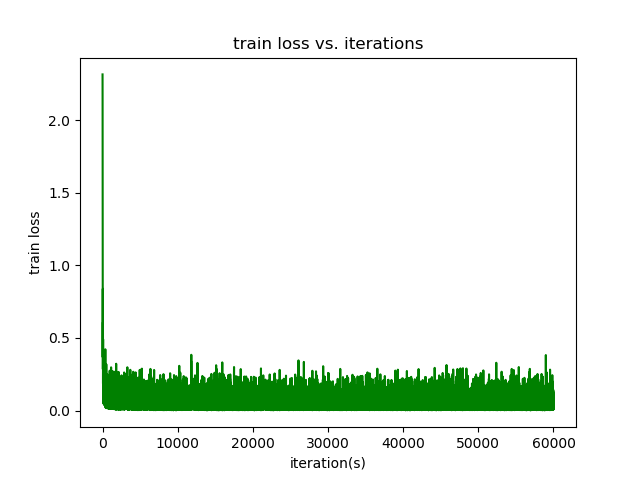
\includegraphics[width=\textwidth]{../results/trainloss21}
	\end{minipage}
	\begin{minipage}[t]{0.48\textwidth}
		\centering
		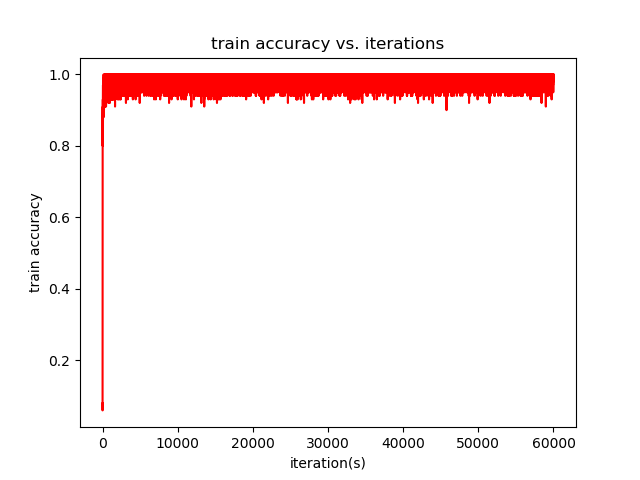
\includegraphics[width=\textwidth]{../results/trainacc21}
	\end{minipage}
	\caption{\label{trainres21}train loss curve and train accuracy curve using CNN with BatchNorm}
\end{figure}

\begin{figure}[!h]
	\centering
	\begin{minipage}[t]{0.48\textwidth}
		\centering
		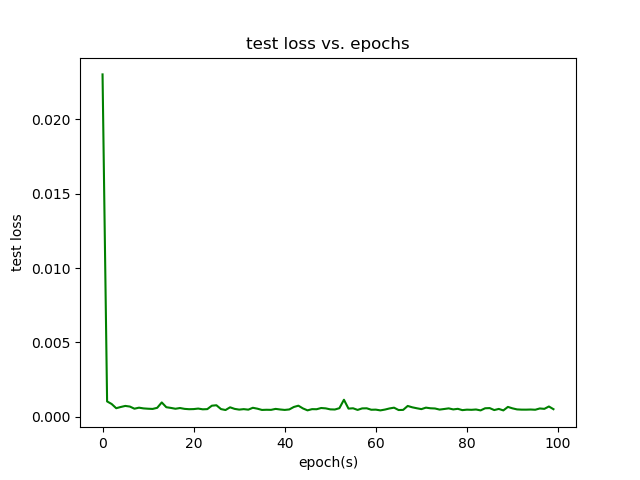
\includegraphics[width=\textwidth]{../results/testloss21}
	\end{minipage}
	\begin{minipage}[t]{0.48\textwidth}
		\centering
		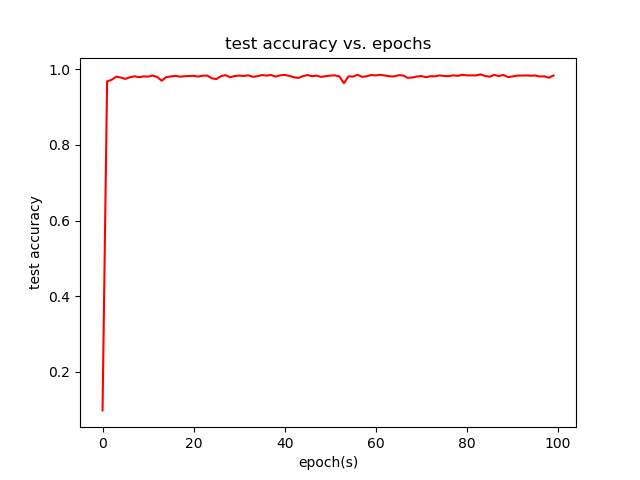
\includegraphics[width=\textwidth]{../results/testacc21}
	\end{minipage}
	\caption{\label{testres21}test loss curve and test accuracy curve using CNN with BatchNorm}
\end{figure}

\subsection{Results without BatchNorm}
From the results we can find that after 35000 iterations, the training accuracy can up to $92\%$, which is slower than the results with BatchNorm, and after one epoch, the test accuracy can up to $95.95\%$, which is also smaller than the results with BatchNorm. Then we draw the train accuracy curve and train loss curve as shown in Figure \ref{trainres22} and we draw the test accuracy curve and test loss curve with respect to epoch as shown in Figure \ref{testres22}.

\begin{figure}[!h]
	\centering
	\begin{minipage}[t]{0.48\textwidth}
		\centering
		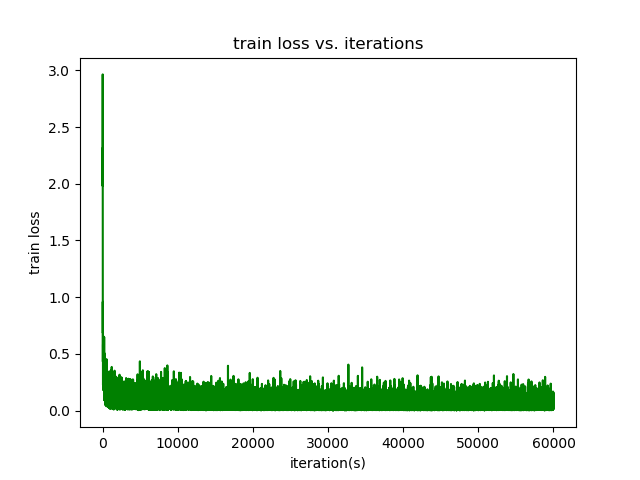
\includegraphics[width=\textwidth]{../results/trainloss22}
	\end{minipage}
	\begin{minipage}[t]{0.48\textwidth}
		\centering
		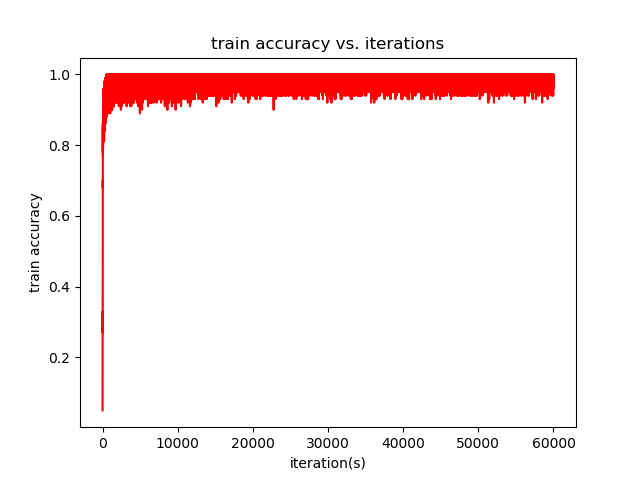
\includegraphics[width=\textwidth]{../results/trainacc22}
	\end{minipage}
	\caption{\label{trainres22}train loss curve and train accuracy curve using CNN without BatchNorm}
\end{figure}

\begin{figure}[!h]
	\centering
	\begin{minipage}[t]{0.48\textwidth}
		\centering
		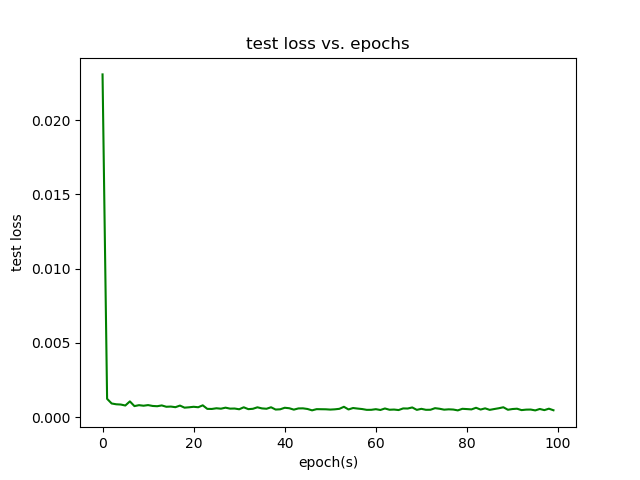
\includegraphics[width=\textwidth]{../results/testloss22}
	\end{minipage}
	\begin{minipage}[t]{0.48\textwidth}
		\centering
		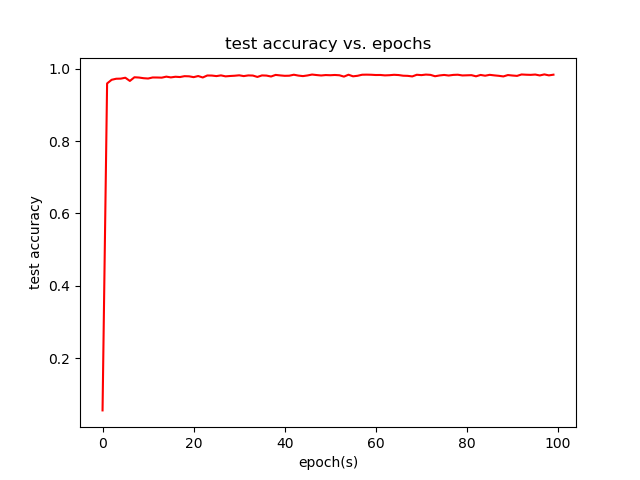
\includegraphics[width=\textwidth]{../results/testacc22}
	\end{minipage}
	\caption{\label{testres22}test loss curve and test accuracy curve using CNN without BatchNorm}
\end{figure}

\subsection{Comparisons}
Here we list the comparisons of the last two results as shown in Table \ref{tab2}. From the table, we can find that:
\begin{itemize}
	\item The result of CNN with BN has faster converging speed than CNN without BN;
	\item The test accuracy and loss of the two experiments is close;
	\item The parameters number of CNN with BN is a little more than CNN without BN, because the BN layer has trainable parameters, but it's a very little number. 
	\item The training time of CNN without BN is a shorter than CNN with BN because CNN with BN has a little more parameters than CNN without BN;
\end{itemize}
Therefore, we can find, using BatchNorm in CNN is better than normal CNN.
\begin{table}[!h]
	\centering
	\caption{\label{tab2}The comparisons of the results with BatchNorm and without BatchNorm}
	\begin{tabular}{|c|c|c|c|c|c|}
		\hline
		Cases & Converge speed & test Acc & test loss & training time & \#(parameters) \\
		\hline
		With BN & faster & 0.983 & 0.0005 & 38min & 2159 \\
		\hline
		Without BN & slower & 0.983 & 0.0005 & 24min & 2143 \\
		\hline
	\end{tabular}
\end{table}

\section{Conclusions}
From the experiments we can find that CNN with BatchNorm has best test accuracy and test loss, and parameters number is small which is not easy to overfit. But the training time is very longer. MLP with BatchNorm has shorter training time and test accuracy is also relatively good. But the parameters number is very large which is easy to result in overfitting. Therefore, choose CNN with BatchNorm is a better way to slove the MNIST digits classification.

\chapter{mini-ResNet}
In this chapter, we design our own mini-ResNet to solve MNIST digits classification task.
\section{ResNet block}
The most important mudule of ResNet is ResNet block, which is shown in Figure \ref{fig3}. From the figure, we can find the forward operation can be computed as follow:
\begin{equation}
y=\mathcal{F}(x)+x
\end{equation}
And the backward operation can be computed by pytorch automaticlly.
\begin{figure}[!h]
	\centering
	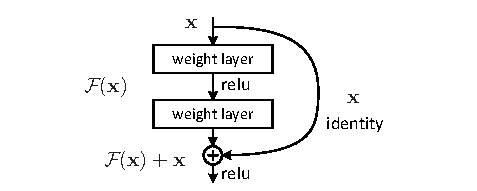
\includegraphics[width=0.8\linewidth]{block.pdf}
	\caption{\label{fig3}Residual learning: a building block}
\end{figure}

The two kinds of ResNet block are shown in Figure \ref{fig4} and in MNIST digits classification task we only use the left one.
\begin{figure}[!h]
	\centering
	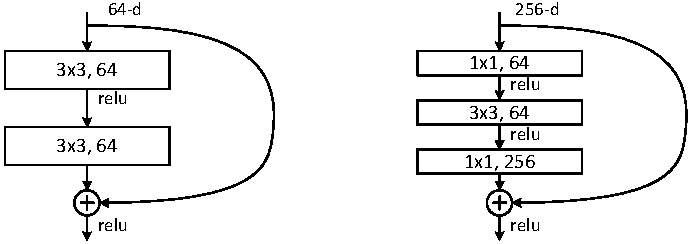
\includegraphics[width=0.8\linewidth]{block_deeper.pdf}
	\caption{\label{fig4}Two kinds of deeper residual function F}
\end{figure}

\section{Network Structure}
Network Structure (eight layers) designed for MNIST digits classification task is shown in Figure \ref{resnet}. Left is the overall structure and right is the detailed structure of one ResNet block.
\begin{figure}[!h]
	\centering
	\begin{minipage}[t]{0.335\textwidth}
		\centering
		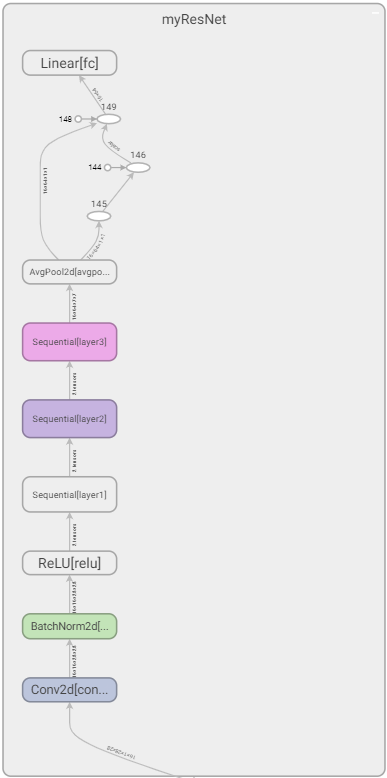
\includegraphics[width=\textwidth]{../results/myresnet1}
	\end{minipage}
	\begin{minipage}[t]{0.65\textwidth}
		\centering
		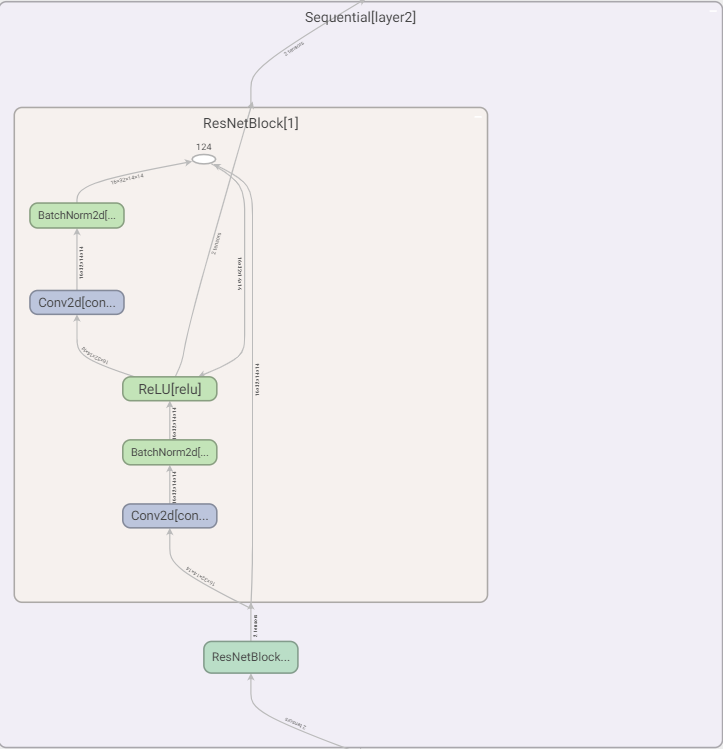
\includegraphics[width=\textwidth]{../results/myresnet2}
	\end{minipage}
	\caption{\label{resnet}MyResNet Network Structure}
\end{figure}

\section{Results}
Only after 5 epochs, test accuracy can up to 99.06\%. We can find it's very powerful. But the training time is too long for my cpu computer. At last, we train for 60 epochs and the best test accuracy is 99.46\% and the best test loss is 0.0004, which is much better than last experiments before. At last we draw the train accuracy curve and train loss curve as shown in Figure \ref{trainres-resnet} and we draw the test accuracy curve and test loss curve with respect to epoch as shown in Figure \ref{testres-resnet}.

\begin{figure}[!h]
	\centering
	\begin{minipage}[t]{0.48\textwidth}
		\centering
		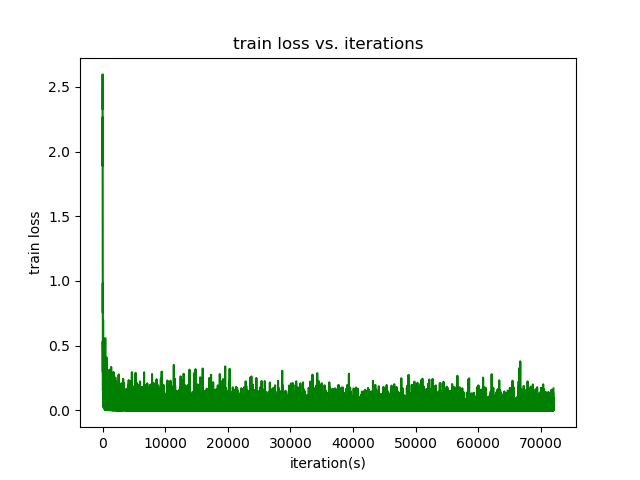
\includegraphics[width=\textwidth]{../results/trainloss-resnet}
	\end{minipage}
	\begin{minipage}[t]{0.48\textwidth}
		\centering
		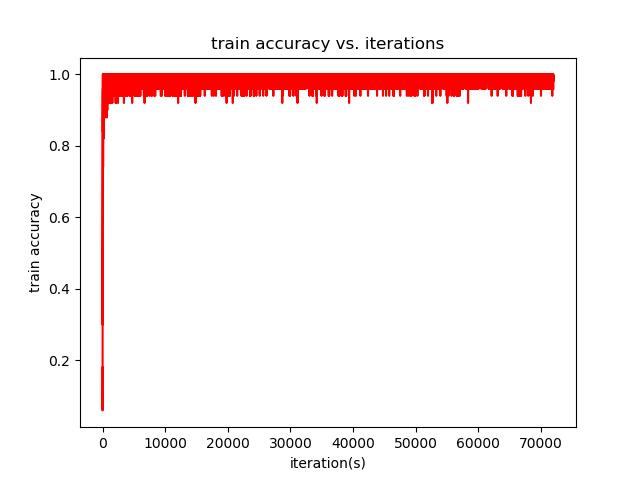
\includegraphics[width=\textwidth]{../results/trainacc-resnet}
	\end{minipage}
	\caption{\label{trainres-resnet}train loss curve and train accuracy curve using mini-ResNet}
\end{figure}

\begin{figure}[!h]
	\centering
	\begin{minipage}[t]{0.48\textwidth}
		\centering
		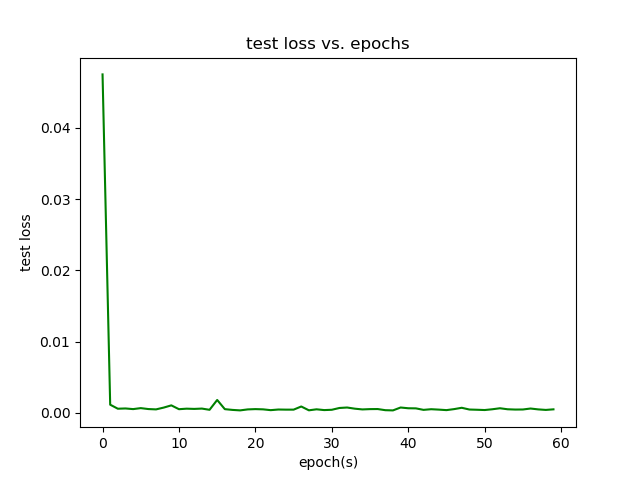
\includegraphics[width=\textwidth]{../results/testloss-resnet}
	\end{minipage}
	\begin{minipage}[t]{0.48\textwidth}
		\centering
		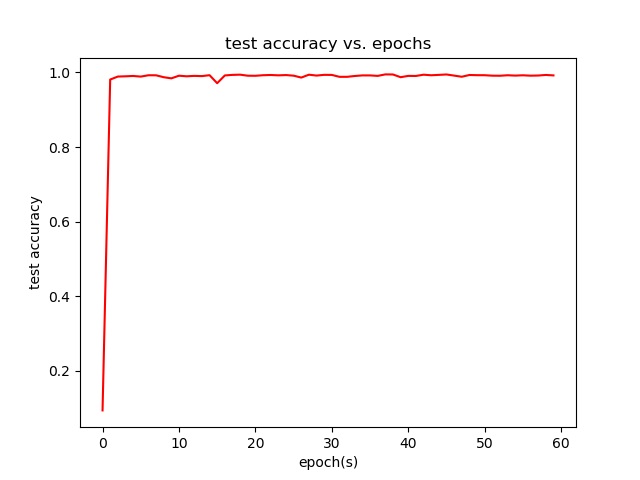
\includegraphics[width=\textwidth]{../results/testacc-resnet}
	\end{minipage}
	\caption{\label{testres-resnet}test loss curve and test accuracy curve using mini-ResNet}
\end{figure}
\end{document}